% document style header
\documentclass[a4paper, 12pt]{config/homework}

% import default packages
\usepackage{config/defpackages}
% import custom math commands
\usepackage{config/domath}
\usepackage{pdfpages}

% end preamble
\begin{document}

% document title
\noindent
\begin{tabularx}{\textwidth}{>{\centering\arraybackslash}X>{\centering\arraybackslash}X>{\centering\arraybackslash}X}
Calvin Sprouse & PHYS489 2B & 2024 February 01\\
\midrule
\end{tabularx}

% Scan your selected artifact(s) and combine these into a single PDF document.
% Prepare a 1/2 page reflection on how the artifact demonstrates your progress to meeting this goal.
% Upload both pdf documents to Canvas by 11:59pm Friday, February 2.


% homework problems begin
\vspace{\baselineskip}
My artifact of choice is a skeletal report from PHYS 333 on a measurement of coaxial transmission line impedance.
Figure 1 of this report shows data collected on the impedance of the transmission line linearized and fit to a model to extract parameters. Applying linear fits to data through computer algorithm is an essential tool for data analysis and enables a more complete understanding of the system than manual approximation.
In this particular experiment a linear model first had to be derived from non-linear data, then corresponding values re-calculated. This was done through Excel sheet and column equations. The corresponding linear fit was also done by calculating the slope, intercept, then using those values to create model data shown in the dashed line.
Determining the slope of the fit represented the impedance of the coax line, which was the goal of the experiment. We compared this experimental measurement to a theoretical impedance calculated from other measured characteristics and found close agreement to 0.490\%. This agreement from two independent sources indicates the linearized model and subsequent fit was preformed correctly. Learning to preform a successful linear fit has benefited nearly every research project I have been involved in, and my methods have become more sophisticated from Excel sheets to Python notebooks.

% insert artifact page
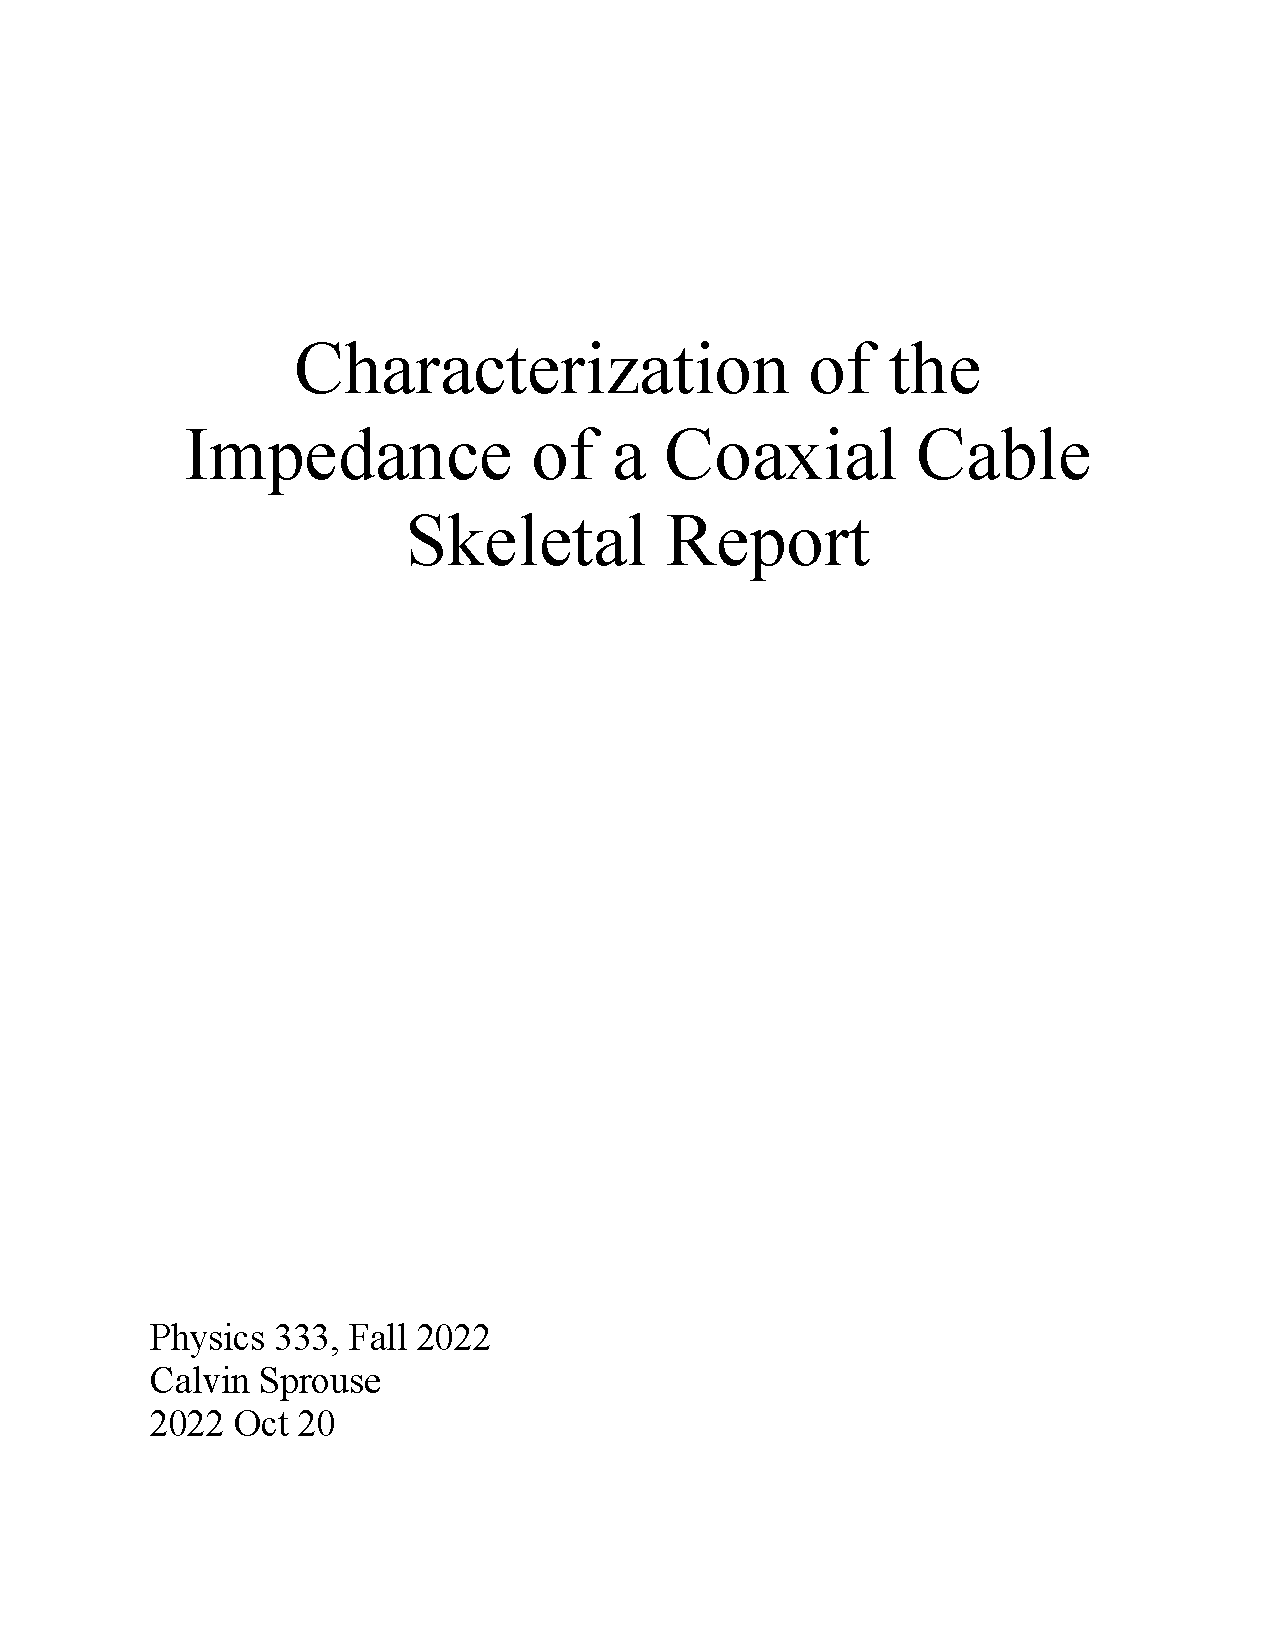
\includepdf[pages=-]{CalvinSprouseCharacterizationOfTransmissionLineImpedanceSkeletal.pdf}
\end{document}
